\chapter{Análisis}

En este capítulo planteo los requisitos funcionales y no funcionales del sistema que he identificado inicialmente y los que han surgido durante su implementación. 
\newline
Así mismo también muestro los actores involucrados en el sistema, un diagrama de los casos de uso y una descripción detallada de cada uno de ellos.



\section{Requisitos Funcionales}
\begin{itemize}
\item \textbf{R.F. 1}. Gestión de Archivos: El sistema debe saber sobre qué archivos debe o no actuar para realizar el análisis del plagio.
	\begin{itemize}
	\item RF 1.1. Se podrán especificar los archivos sobre los que se quiera saber si hay plagio.
	\item RF 1.2. El sistema sabrá reconocer los archivos con extensión .r y .R
	\item RF 1.3. El sistema tiene a R como opción de ejecución para aplicar la detección sobre archivos en este lenguaje. 
	\item RF 1.4. El sistema ignorará los archivos no válidos (que no sean del lenguaje especificado) o con errores.
	\end{itemize}
\item \textbf{R.F. 2}. Gestión de Resultados: El sistema deberá de gestionar los resultados obtenidos de aplicar el algoritmo de JPLAG a los archivos.
	\begin{itemize}
	\item RF 2.1. El sistema guardará los resultados en el directorio que se le especifique.
	\item RF 2.2. El sistema creará los subdirectorios necesarios en caso de no existir la ruta al directorio en el que almacenar los resultados.
	\item RF 2.3. El sistema mostrará los resultados de la ejecución en terminal en todo momento.
	\end{itemize}
\end{itemize}


\section{Requisitos No Funcionales}
\begin{itemize}
\item \textbf{R.N.F. 1}. Eficiencia.
El frontend implantado no deberá demorar en su uso al sistema más que el resto de los frontends para el resto de lenguajes.
\item \textbf{R.N.F. 2}. Eficacia.
El frontend implantado tendrá que obtener resultados iguales o mejores que el resto de frontends con archivos de código en R.
\item \textbf{R.N.F. 3}. Extensivilidad.
El frontend implantado tendrá que ser fácilmente modificable para poder probar con otros tokens del lenguaje.
\end{itemize}

\section{Actores}

\begin{figure}[H] %con el [H] le obligamos a situar aquí la figura
\centering
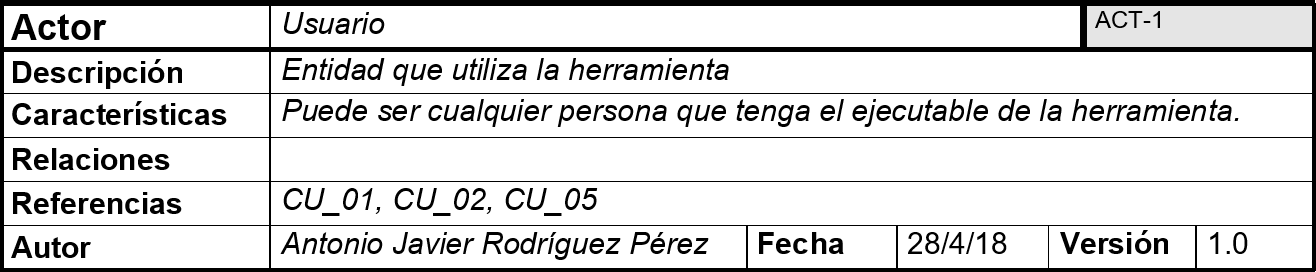
\includegraphics[scale=0.4]{imagenes/ACT_1.png}  %el parámetro scale permite agrandar o achicar la imagen. En el nombre de archivo puede especificar directorios
\caption{Actor 1} \label{fig:figura2}
\end{figure}

\begin{figure}[H] %con el [H] le obligamos a situar aquí la figura
\centering
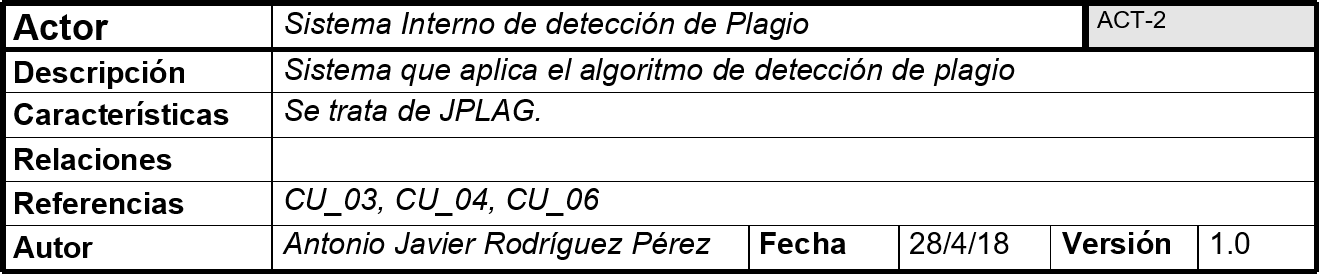
\includegraphics[scale=0.4]{imagenes/ACT_2.png}  %el parámetro scale permite agrandar o achicar la imagen. En el nombre de archivo puede especificar directorios
\caption{Actor 2} \label{fig:figura3}
\end{figure}



\section{Diagrama de Casos de Uso}

\begin{figure}[H] %con el [H] le obligamos a situar aquí la figura
\centering
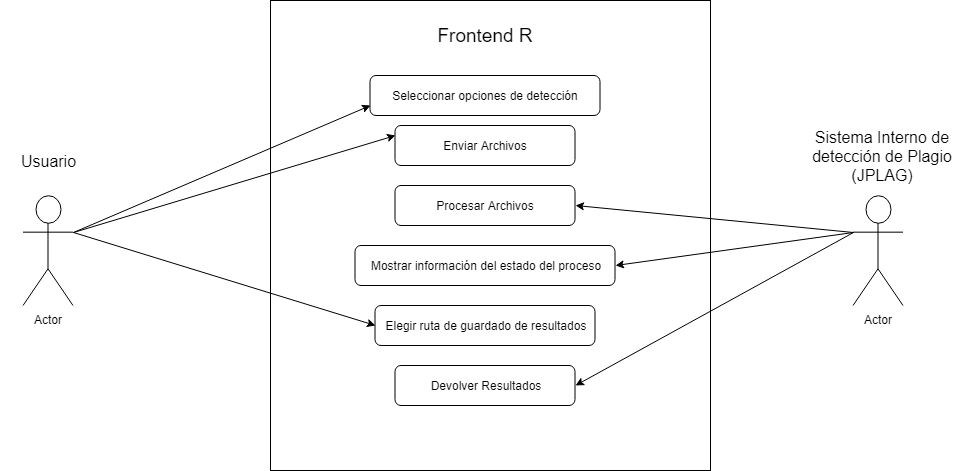
\includegraphics[scale=0.45]{imagenes/Diagrama_CU.png}  %el parámetro scale permite agrandar o achicar la imagen. En el nombre de archivo puede especificar directorios
\caption{Diagrama de casos de uso del usuario del sistema.} \label{fig:figura4}
\end{figure}

\section{Casos de Uso}

\begin{figure}[H] %con el [H] le obligamos a situar aquí la figura
\centering
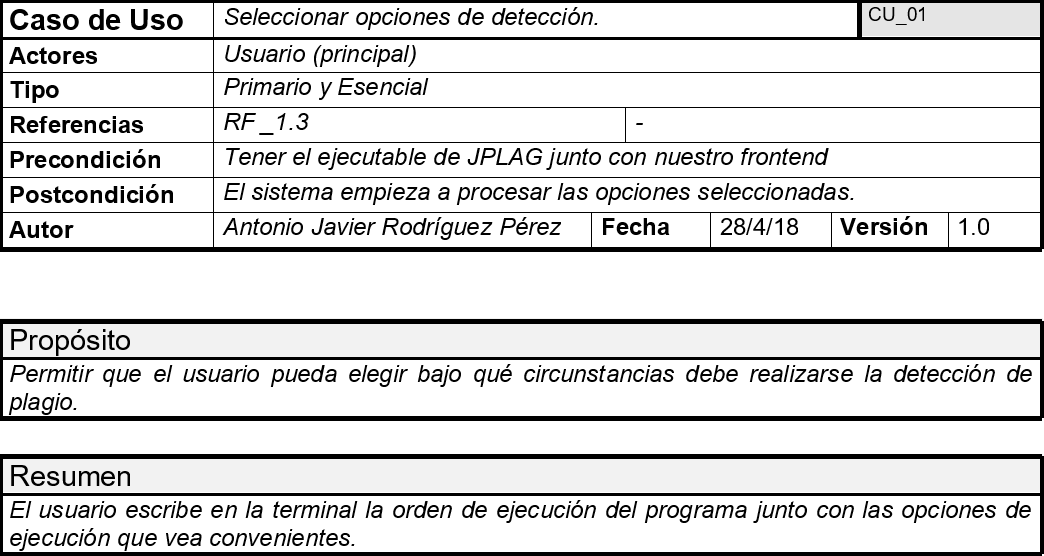
\includegraphics[scale=0.5]{imagenes/CU_01.png}  %el parámetro scale permite agrandar o achicar la imagen. En el nombre de archivo puede especificar directorios
\caption{Caso de uso 1.} \label{fig:CU1}
\end{figure}

\begin{figure}[H] %con el [H] le obligamos a situar aquí la figura
\centering
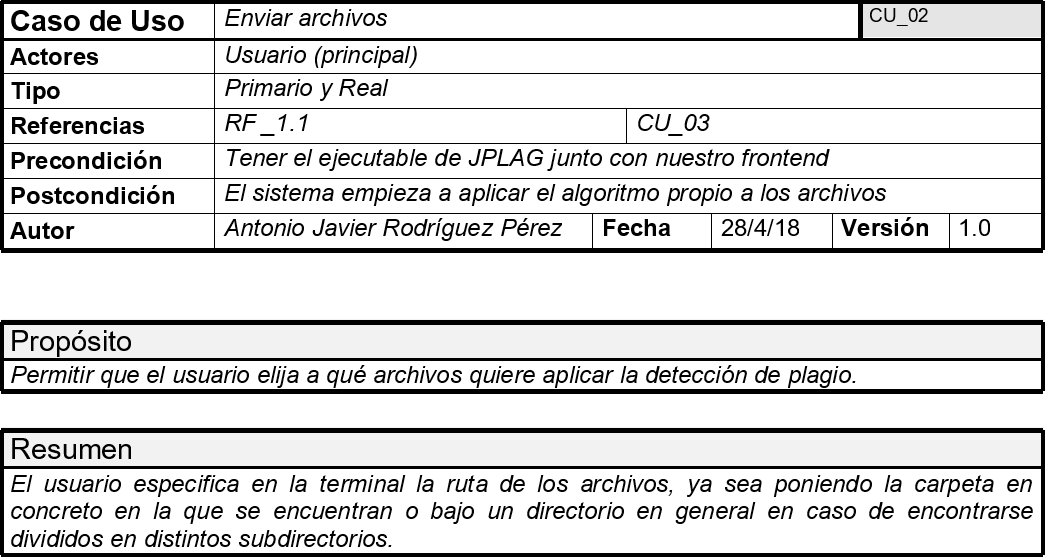
\includegraphics[scale=0.5]{imagenes/CU_02.png}  %el parámetro scale permite agrandar o achicar la imagen. En el nombre de archivo puede especificar directorios
\caption{Caso de uso 2.} \label{fig:CU2}
\end{figure}

\begin{figure}[H] %con el [H] le obligamos a situar aquí la figura
\centering
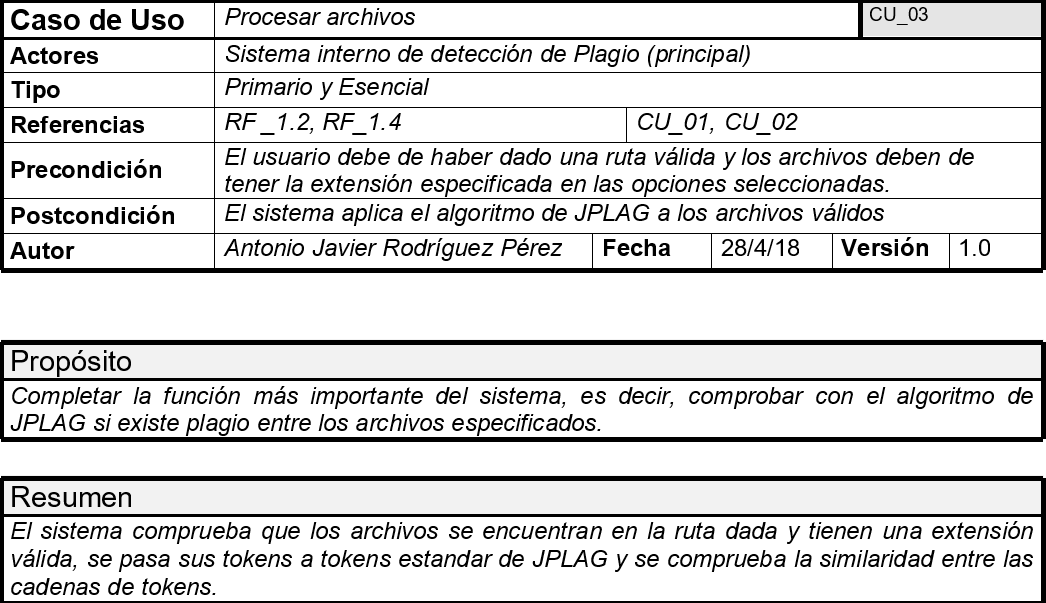
\includegraphics[scale=0.5]{imagenes/CU_03.png}  %el parámetro scale permite agrandar o achicar la imagen. En el nombre de archivo puede especificar directorios
\caption{Caso de uso 3.} \label{fig:CU3}
\end{figure}

\begin{figure}[H] %con el [H] le obligamos a situar aquí la figura
\centering
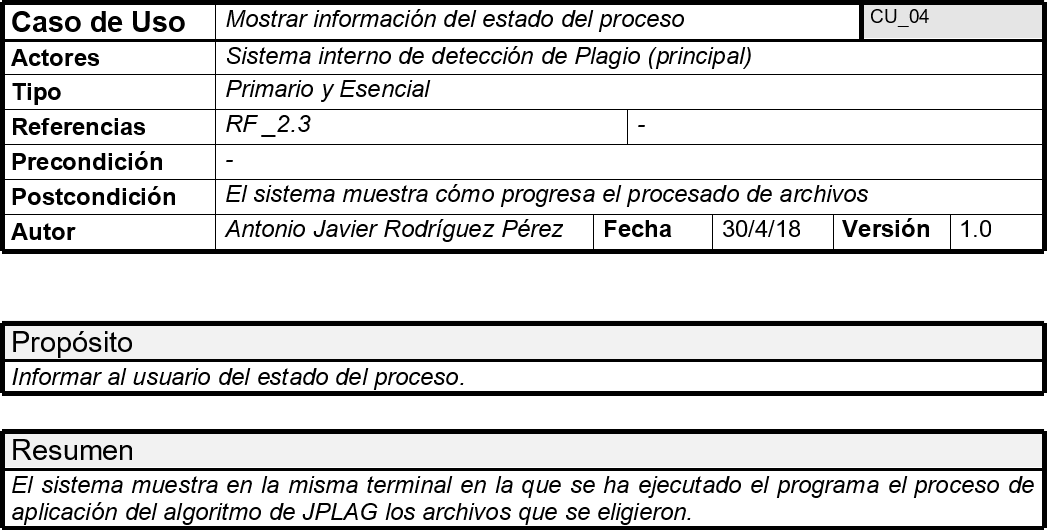
\includegraphics[scale=0.5]{imagenes/CU_04.png}  %el parámetro scale permite agrandar o achicar la imagen. En el nombre de archivo puede especificar directorios
\caption{Caso de uso 4.} \label{fig:CU4}
\end{figure}

\begin{figure}[H] %con el [H] le obligamos a situar aquí la figura
\centering
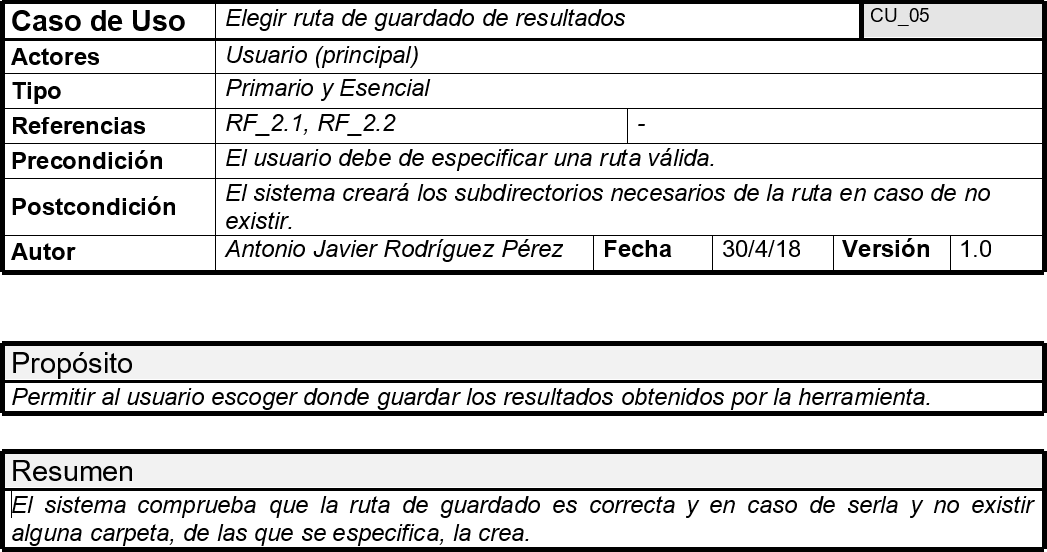
\includegraphics[scale=0.5]{imagenes/CU_05.png}  %el parámetro scale permite agrandar o achicar la imagen. En el nombre de archivo puede especificar directorios
\caption{Caso de uso 5.} \label{fig:CU5}
\end{figure}

\begin{figure}[H] %con el [H] le obligamos a situar aquí la figura
\centering
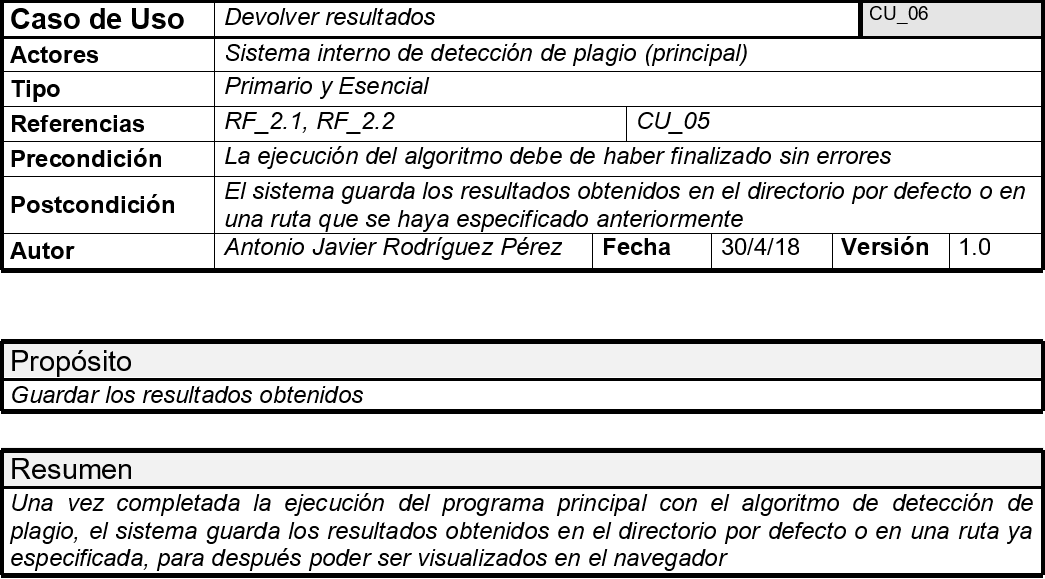
\includegraphics[scale=0.5]{imagenes/CU_06.png}  %el parámetro scale permite agrandar o achicar la imagen. En el nombre de archivo puede especificar directorios
\caption{Caso de uso 6.} \label{fig:CU6}
\end{figure}

